%!TEX root = /Users/audrey/Dropbox/PhD/MOMAB/ArXiv/Latex/paper.tex

\section{Preference Radius}
\label{sec:preference_radius}

Let $\bstheta_a(t)$ denote the estimation associated with action $a$ on episode $t$ and let $\cP(t) = \{ a : \nexists \bstheta_b(t) \succ \bstheta_a(t) \}_{a, b \in \cA}$ denote the estimated Pareto front given these options. By definition, the optimal options are $\cO(t) \subseteq \cP(t)$. Let
\begin{align*}
    B(\bsc, r) \subseteq \{ \bsx \in \cX : |x_i - c_i| < r, ~ i = 1, \dots, d \}
\end{align*}
denote a ball of center $\bsc$ and radius $r$. In order to characterize the difficulty of a multi-objective bandits setting, we introduce the following quantity.
%
\begin{definition}
For each action $a \in \cA$, we define the preference radius $\rho_a$ as any radius such that if $\bstheta_a(t) \in B(\bsmu_a, \rho_a)$ for all actions, then
\begin{align*}
    \exists \star \in \cO : \star \in \cO(t) \quad \text{and} \quad a \not\in \cO(t) ~ \forall a \in \cA, a \not\in \cO.
\end{align*}
\end{definition}
%
The radii correspond to the \emph{robustness} of the preference function, that is to which extent can actions be poorly estimated simultaneously before the set of optimal options changes. The radius $\rho_a$ is directly linked to the gap $\Delta_a = f(\bsmu_\star)- f(\bsmu_a)$. For a suboptimal action, a large radius indicates that this action is far from being optimal. Also, the preference radii of suboptimal actions depend on the preference radius of the optimal action(s). Larger optimal action radii imply smaller radii for suboptimal actions. Note that if all actions estimates stand in their preference balls, being greedy is optimal.

Let $\alpha_1, \dots, \alpha_d \in [0, 1]$ denote \emph{weights} such that $\sum_{i = 1}^d \alpha_i = 1$. The weighted $L_p$ metric $f(\bsx)= \big( \sum_{i = 1}^d \alpha_i x_i^p \big)^{1/p}$ with $p \geq 1$ is often used to represent decision functions. This function is known as the linear scalarization when $p = 1$ and as the Chebyshev scalarization when $p = \infty$. The following examples show the link between the preference radii and the gap for these two common functions.

\begin{figure}[t]
    \centering
    \begin{subfigure}[b]{0.35\textwidth}
        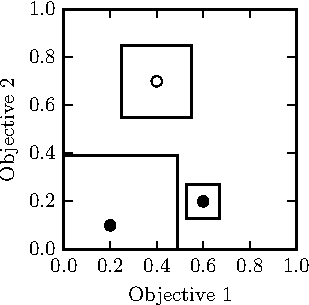
\includegraphics[scale=0.75]{pref_radius_weighted_sum_2}
    \end{subfigure}
    \qquad
    \begin{subfigure}[b]{0.35\textwidth}
        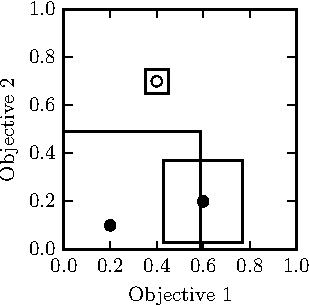
\includegraphics[scale=0.75]{pref_radius_weighted_sum_1}
    \end{subfigure}
    \caption{Examples of preference radii around the optimal (white) and suboptimal (black) actions given the linear preference function $f(\bsx) = 0.4 x_1 + 0.6 x_2$.}
\label{fig:pref_radius:example:weigthed_sum}
\end{figure}

\begin{example}[Linear]
\label{ex:linear}
    The linear scalarization function is given by
    \begin{align*}
        f(\bsx) = \sum_{i = 1}^d \alpha_i x_i.
    \end{align*}
    Consider the optimal action $\star$ and the suboptimal action $a$. By definition of the preference radii, we have that
    \begin{align*}
        \min_{\bstheta_\star \in B(\bsmu_\star, \rho_\star)} f(\bstheta_\star) & > \max_{\bstheta_a \in B(\bsmu_a, \rho_a)} f(\bstheta_a) \\
        \sum_{i = 1}^d (\alpha_i \mu_{\star, i} - \alpha_i \rho_\star) &> \sum_{i = 1}^d (\alpha_i \mu_{a, i} + \alpha_i \rho_a) \\
        f(\bsmu_\star) - \rho_\star & > f(\bsmu_a) + \rho_a \\
        \Delta_a & > \rho_\star + \rho_a.
    \end{align*}
    Fig.~\ref{fig:pref_radius:example:weigthed_sum} shows examples of preference radii with a linear preference function.
%In both cases, as long as each option stays in its associated radius, the expert user preference won't change.
\end{example}

\begin{example}[Chebyshev]
\label{ex:chebyshev}
    The Chebyshev scalarization~\cite{Bowman1976} function is given by
    \begin{align*}
        f(\bsx) = \max_{1 \leq i \leq d} \alpha_i x_i.
    \end{align*}
    Consider the optimal and suboptimal actions $\star$ and $a$, and let
    \begin{align*}
        i_\star = \argmax_{1 \leq i \leq d} \alpha_i (\mu_{\star, i} - \rho_\star), \quad
        i_a = \argmax_{1 \leq i \leq d} \alpha_i (\mu_{a, i} - \rho_a).
    \end{align*}
    By definition of the preference radii, we have that
    \begin{align*}
        \min_{\bstheta_\star \in B(\bsmu_\star, \rho_\star)} f(\bstheta_\star) & > \max_{\bstheta_a \in B(\bsmu_a, \rho_a)} f(\bstheta_a) \\
        \max_{1 \leq i \leq d} \alpha_i (\mu_{\star, i} + \rho_\star) & > \max_{1\leq i \leq d} \alpha_i (\mu_{a, i} - \rho_a) \\
        \alpha_{i_\star} \mu_{\star, i} - \alpha_{i_\star} \rho_\star & > \alpha_{i_a} \mu_{a, i} + \alpha_{i_a} \rho_a  \\
        f(\bsmu_\star) - \alpha_{i_\star} \rho_\star &> f(\bsmu_a) + \alpha_{i_a} \rho_a \\
        \Delta_a &> \alpha_{i_\star} \rho_\star + \alpha_{i_a} \rho_a.
    \end{align*}
    The difficulty here is that $i_\star$ and $i_a$ respectively depend on $\rho_\star$ and $\rho_a$. Consider a 2-objective setting, we can define
    \begin{align*}
        \tau_\star = \frac{\alpha_2 \mu_{\star, 2} - \alpha_1 \mu_{\star, 1}}{\alpha_2 - \alpha_1}, \quad
        \tau_a = \frac{\alpha_1 \mu_{a, 1} - \alpha_2 \mu_{a, 2}}{\alpha_2 - \alpha_1}
    \end{align*}
    as thresholds such that
    \begin{align*}
        i_\star = \bigg\{
            \begin{array}{ll}
            1 & \quad \text{if} \quad \rho_\star > \tau_\star \\
            2 & \quad \text{otherwise}
            \end{array}, \quad
        i_a = \bigg\{
            \begin{array}{ll}
            1 & \quad \text{if} \quad \rho_a < \tau_a \\
            2 & \quad \text{otherwise}.
            \end{array}
    \end{align*}
    %
    Fig.~\ref{fig:pref_radius:example:chebyshev} shows examples of preference radii with a Chebyshev preference function. 
\end{example}

\begin{figure}[t]
    \centering
    \begin{subfigure}[b]{0.35\textwidth}
        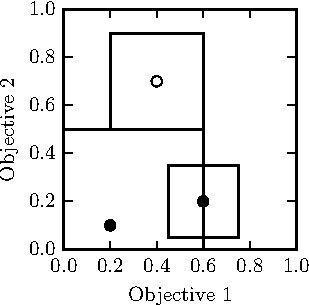
\includegraphics[scale=0.75]{pref_radius_chebyshev_2}
    \end{subfigure}
    \qquad
    \begin{subfigure}[b]{0.35\textwidth}
        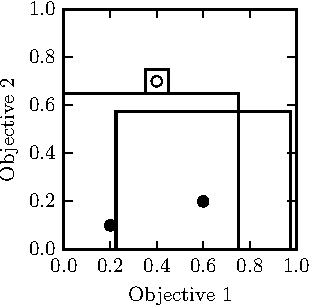
\includegraphics[scale=0.75]{pref_radius_chebyshev_1}
    \end{subfigure}
    \caption{Examples of preference radii around the optimal action (white) and suboptimal actions (black) given a Chebyshev function with $\alpha_1 = 0.4$ and $\alpha_2 = 0.6$.}
\label{fig:pref_radius:example:chebyshev}
\end{figure}

Outside $L_p$ metrics, other scalarization functions are often based on constraints. For example, using the $\epsilon$-constraint scalarization technique, a user assigns a constraint to every objective except a target objective $\ell$. All options that fail to respect one of the contraints receive a value of 0, while the options that respect all constraints get a value of $x_\ell$. The following example shows the relation between the preference radius and the gap given a preference function that is articulated as an $\epsilon$-constraint scalarization technique.
%
\begin{example}[Epsilon-constraint]
\label{ex:epsilon-constraint}
    The $\epsilon$-constraint function is given by
    \begin{align*}
    f(\bsx) = \bigg\{
        \begin{array}{ll}
        x_\ell & \quad \text{if} \quad x_i \geq \epsilon_i \quad \forall i \in \{ 1, \dots, d \}, i \neq \ell \\
        0 & \quad \text{otherwise}.
        \end{array}
    \end{align*}
    Consider the optimal and suboptimal actions $\star$ and $a$. By definition of the preference radii, we have that
    \begin{align*}
        \rho_\star \leq \min_{1 \leq i \leq d, i \neq \ell} \mu_{\star, i} - \epsilon_i.
    \end{align*}
    We decompose $\rho_a = \ubar{\rho}_a + \bar{\rho}_a$ such that
    \begin{align*}
        \ubar{\rho}_a = \min \{ 0, \max_{1 \leq i \leq d, i \neq \ell} \epsilon_i - \mu_{a, i} \}
    \end{align*}
    denotes the radius required in order for action a to respect the constraints, that is to obtain $f(\bsmu_a) > 0$, and $\bar{\rho}_a$ denotes the leftover leading to a gap reduction. Finally, we have that
    \begin{align*}
        \mu_{\star, \ell} - \rho_\star > \mu_{a, \ell} + \ubar{\rho}_a + \bar{\rho_a} \quad \text{and} \quad
        \Delta_a > \rho_\star + \rho_a.
    \end{align*}
    Fig.~\ref{fig:pref_radius:example:econstraint} shows examples of preference radii with $\epsilon$-constraint preference functions.
\end{example}

\begin{figure}[t]
    \centering
    \begin{subfigure}[b]{0.35\textwidth}
        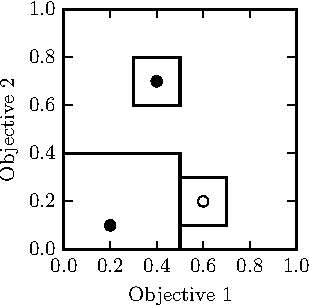
\includegraphics[scale=0.75]{pref_radius_econstraint_f2}
        \caption{$\ell = 1$, $\epsilon_2 = 0.1$}
    \end{subfigure}
    \qquad
    \begin{subfigure}[b]{0.35\textwidth}
        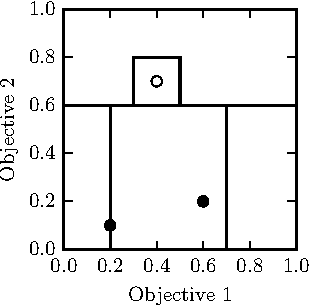
\includegraphics[scale=0.75]{pref_radius_econstraint_f1}
        \caption{$\ell = 2$, $\epsilon_1 = 0.3$}
    \end{subfigure}
    \caption{Examples of preference radii around the optimal (white) and suboptimal (black) actions given two different configurations of $\epsilon$-contraint.}
\label{fig:pref_radius:example:econstraint}
\end{figure}
